\lezione{16}{09.05.17}

\section{Vettori aleatori}
La trattazione dei \emph{vettori aleatori} è una parte fondamentale dello studio della probabilità: essi rappresentano infatti il caso più generale e utilizzato delle variabili aleatorie.
Parte del capitolo servirà per reintrodurre la teoria precedentemente sviluppata sulle variabili monodimensionali, che si manterrà sostanzialmente tale e quale nel passaggio da $\RR$ a $\RR^n$.
Sarà inoltre introdotta la \emph{covarianza}, che indica il legame probabilistico tra le componenti del vettore; da essa discenderà il \emph{coefficiente di correlazione lineare}, molto utile anche in ambito statistico.

\index{vettore aleatorio}
I \textbf{vettori aleatori} sono variabili aleatorie a valori in $(\RR^n, \Bc^n)$, ovvero:
$$X = (x_1 \dots x_n) = \begin{pmatrix} x_1 \\ \vdots \\ x_n \end{pmatrix} = [x_1 \dots x_n] = \begin{bmatrix} x_1 \\ \vdots \\ x_n \end{bmatrix} : \DoCo$$
Nel testo saranno usate interscambiabilmente la notazione colonna e quella riga e le parentesi tonde e quadre, a seconda della convenienza estetica del momento.\footnote{Ciò non toglie che se usi le tonde sei una brutta persona}

Sappiamo già che:
\begin{itemize}
  \item $\Bc^n = \sigma(\tau^n) = \Bc^{\bigotimes n} = \sigma \left( \bigtimes\limits_{k = 1}^{n} (-\infty, t_k] : t_k \in \QQ \right)$

    In quest'ultima scrittura gli insiemi generanti sono detti \emph{iper-quadranti} di sud-ovest, già visti nell'esempio a pagina \pageref{ese-iperquadranti}.
  \item $X$ misurabile $\iff X_k$ misurabili $\forall k$; ovvero, non ci sono problemi o perdite di misurabilità passando dal vettore alle componenti e viceversa.
  \item Se $X: \Omega \to \RR^n$ è misurabile e $h: \RR^n \to \RR^k$ è boreliana, allora $Y = h(X): \Omega \to \RR^k$ è misurabile.
  \item $X \aceq Y \iff X_k \aceq Y_k \;  \forall k$.
  \item $P^X$ dipende solo da $[X]$, la \emph{classe di equivalenza} della variabile $X$.
  \item Se $X_1, X_2 \in L^2$, allora $X_1 \cdot X_2 \in L^1$ e vale la \emph{disuguaglianza di Cauchy-Schwarz}:
  $$ | \Ex{X_1 X_2} | \leq \sqrt{\Ex{X_1^2} \, \Ex{X_2^2}}$$
  \item Se $X_1, X_2$ sono in $L^1$ e $X_1 \indep X_2$, allora $X_1 X_2 \in L^1$.
  \item Si ha la seguente serie di equivalenze: $X_1 \indep X_2$
  \begin{itemize}
    \item[] $\iff  \PP(X_1 \in A, X_2 \in B) = \PP_1(X_1 \in A) \PP_2(X_2 \in B) \ \ \forall A \in \Cc, \ \forall B \in \Dc$ \\
        con $\sigma(\Cc) = \sigma(\Dc) = \Bc$ e $\Cc,\Dc$ chiusi per intersezioni finite

    \item[] $\iff h(X_1) \indep g(X_2) \ \forall h, \forall g$ misurabili

    \item[] $\iff \Ex{h(X_1) g(X_2)} = \Ex{h(X_1)} \Ex{g(X_2)}$ \\
        $\forall h, \forall g$ misurabili e positive, misurabili e limitate, oppure continue e limitate

    \item[] $\iff P^{(X_1, X_2)} = P^{X_1} \otimes P^{X_2}$.
  \end{itemize}
  \begin{nb}
    L'ultima condizione è la più facile da verificare e la più utilizzata nelle applicazioni pratiche.
  \end{nb}
\end{itemize}

\medskip
\begin{defn}
  \index{funzione!di ripartizione in $\RR^n$}
  $F_X: \RR^n \to [0,1]$ è detta \textbf{funzione di ripartizione} in $\RR^n$ se:
  $$F_X (t) = F_X(t_1, \, \dots, \, t_n) \coloneqq \PP(X_1 \leq t_1, \, \dots, \, X_n \leq t_n) = \PP \left( X \in \bigtimes_{k=1}^n (-\infty,t_k] \right)$$
  Equivalentemente, $F_X(t_1, \, \dots, \, t_n)$ è la probabilità che $X$ sia in un iper-quadrante di sud-ovest delimitato dai valori $t_k$ assegnati.
\end{defn}
Nel caso generale di $n \geq 2$ la definizione risulta spesso complicata, quindi si tenterà di farne a meno nei successivi sviluppi della teoria.

\subsection[Vettori aleatori discreti]{Vettori aleatori discreti\footnote{La trattazione dei vettori aleatori discreti non è presente sullo J-P; evidentemente pensavano (sbagliando) che fosse possibile arrivarci da soli a questo punto del corso.}}

\begin{defn}
  \index{densità di probabilità!discreta}
  La funzione positiva $p: S \to [0,1]$, con $S$ al più numerabile,
  è detta \textbf{densità discreta di probabilità} se:
  $$\sum_{x \in S} p(x) = 1 \quad \text{e} \quad P^X(B) = \sum_{x \in S \cap B} p(x)$$
\end{defn}

\begin{defn}
  \index{vettore aleatorio!discreto}
  Sia $\Dom$ uno spazio di probabilità e $X: \Omega \to \RR^n$ misurabile. \\
  $X$ è detto \textbf{vettore aleatorio discreto} se la sua legge $P^X$ è discreta su $\Bc^n$, ovvero
  esiste un insieme discreto $S$, al più numerabile, su cui è definita una
  densità discreta di probabilità $p: S \to [0,1]$.
\end{defn}
Si noti che la definizione non riguarda il dominio di $X$ ma solamente il codominio, ovvero la legge $P^X$. Si noti inoltre che la definizione non esclude la possibilità che $S$ contenga punti a probabilità nulla, i quali sono ``inutili'' nella costruzione della legge. Per questo motivo $S$ non è univocamente determinato, anche se, quando c'è possibilità di scegliere, molto spesso si prende $S$ contenente solo punti con probabilità positiva, per evitare ridondanze e garantire comunque l'unicità di $S$.\\
\vspace{-\baselineskip}

\subsubsection{Condizioni equivalenti}
Le seguenti affermazioni sono equivalenti:
\begin{itemize}
  \item $X$ è vettore aleatorio discreto;
  \item $\exists \ S \subset \RR^n$, al più numerabile, tale che $\PP(X \in S) = 1$;
  \item $\im(X) = S$ al più numerabile a meno di elementi trascurabili, ovvero $X \aceq \widetilde{X}$ con $\im(\widetilde{X}) = S$ al più numerabile;
   (per esempio, $\widetilde{X} = X \Ind_S (X) + x_0 \Ind_{S^C} (X)$ con $x_0$ arbitrario, e comunque irrilevante in quanto è raggiunto da $X$ con probabilità nulla)
  \item $X_1, \, \dots, \, X_n$ VA \emph{discrete}.
\end{itemize}


Dimostriamo ora la coimplicazione ``$X$ vettore aleatorio discreto $\iff$ $X_1, \, \dots, \, X_n$ VA discrete'', che è di gran lunga la più importante: è facile da verificare ed è peculiare dei vettori discreti (si vedrà più avanti che questa equivalenza non è valida nel caso continuo).

\begin{dimo}
  \Fixvmode
  \begin{itemize}
    \item \textbf{($\implies$)}:
    \begin{figure}[h]
      \centering
      \begin{tikzpicture}
      \begin{axis}[
          axis lines = middle,
          xlabel = $X$,
          ylabel = $Y$,
          width=0.5\textwidth,
      ]

      \draw [line width=0.2mm, dashed] (axis cs:0,1) -- (axis cs:3,1) -- (axis cs:3,0);
      \draw [line width=0.2mm, dashed] (axis cs:0,2) -- (axis cs:2,2) -- (axis cs:2,0);
      \draw [line width=0.2mm, dashed] (axis cs:0,3) -- (axis cs:1,3) -- (axis cs:1,0);

      \addplot [only marks, mark=*] table {
      3 1
      2 1
      2 2
      1 3
      };

      \addplot [draw=none, forget plot] coordinates {(3.5, 3.5)};
      \addplot [draw=none, forget plot] coordinates {(0, 0)};
      \end{axis}
      \end{tikzpicture}
      \caption{proiezione di un vettore aleatorio di dimensione 2}
    \end{figure}

    Se $X$ è discreto, $\exists \ S$ discreto tale che $\PP (X \in S) = 1$. Sia ora $S_k$ la \emph{proiezione} di $S$ sull'asse $X_k$ (per definirla in astratto è necessario un prodotto scalare, ma una definizione geometrica è sufficiente per l'intuizione). \\
    Poiché $X \in S \implies X_k \in S_k$, si ha la relazione tra eventi $(X_k \in S_k) \supseteq (X \in S)$: dunque
    $\PP(X_k \in S_k) \geq \PP(X \in S) \stackrel{\text{hp}}{=} 1$. Ma allora $\PP(X_k \in S_k) = 1$, che è la tesi. \\

    \item \textbf{($\impliedby$)}:
    per ipotesi esistono $S_1, \, \dots, \, S_n$, supporti al più numerabili di $X_1, \, \dots, \, X_n$. \\
    Si definisca la seguente \emph{griglia}:
    $$S = \bigtimes\limits_{k=1}^n S_k$$
    Essa è un insieme $n$-rettangolare nel quale sono sicuramente racchiusi tutti i punti di $X$ su cui è concentrata la probabilità, più un numero indefinito di punti a probabilità nulla (che comunque non ostruiscono la dimostrazione). Dunque:
    $$ \Omega \supseteq (X \in S) = \bigcap_{k=1}^n (X_k \in S_k) \implies
    \PP(X \in S) = \PP \left( \bigcap_{k=1}^n (X_k \in S_k) \right)$$
    Tutti gli eventi dell'intersezione hanno probabilità 1, pertanto anche la loro intersezione $S$ ha probabilità 1. \qedhere
  \end{itemize}
\end{dimo}

\subsubsection{Legge congiunta e legge marginale}

\index{legge!congiunta}
\index{legge!marginale}
Cerchiamo ora un legame tra la legge $P^X$ di $X$, detta \textit{legge congiunta}, e le leggi $P^{X_k}$ delle $X_K$, dette \textit{leggi marginali}.
\begin{prop}
  Sia $X$ vettore aleatorio discreto con densità $p$ sul supporto $S = \bigtimes\limits_{k=1}^n S_k$. \\
  Allora la VA $X_k$ ha densità discreta:
  $$p_k(x_k) = \sum_{ \substack
    {x_1 \in S_1 \\ \dots \\
    x_{k-1} \in S_{k-1} \\
    x_{k+1} \in S_{k+1} \\ \dots \\
    x_n \in S_n}}
  p(x_1, \, \dots, \, x_n)$$
\end{prop}

In altre parole, chiedendo la legge marginale di $X_k$, stiamo tenendo fisso il valore di $X_k$ e stiamo facendo la somma dei termini della legge congiunta \emph{al variare di tutte le coordinate che \textbf{non} sto sommando}, ovvero tutte tranne $X_k$.

\begin{dimo}
  Per semplicità di notazione sarà dimostrato solo il caso $n = 2$; il caso generale è analogo. \\
  Si definisca $p_1$ nel seguente modo, che può essere riscritto grazie alla formula delle probabilità totali:
  $$p_1(x_1) \coloneqq \PP(X_1 = x_1) = \sum_{x_2 \in S_2} \PP(X_1 = x_1, X_2 = x_2) = \sum_{x_2 \in S_2} p(x_1, x_2)$$
  Ciò è possibile in quanto gli eventi della forma $(x_k \in S_k)$ formano una partizione di $S$ (ancora, coprire tutto $\Omega$ non è necessario in quanto fuori da $S$ esistono solo punti a probabilità nulla). Similmente si ricava anche $p_2(x_2)$.
\end{dimo}

\subsubsection{Valore atteso per vettori discreti}

\begin{prop}[regola del valore atteso]
  \index{valore atteso!per vettori discreti}
  Siano $X: \DoCo$ un vettore aleatorio discreto con densità $p$ e $h:\RR^n \to \RR$ una funzione misurabile, con $h$ positiva oppure in $L^1(P^X)$. Allora:
  $$ \Ex{h(X)} = \int_\Omega h(X) \, \dPP = \int_{\RR^n} h(x) \, \de P^X \stackrel{\downarrow}{=} \sum_{x \in S} h(x) \, p(x)$$
\end{prop}
La dimostrazione è simile a quella per le precedenti versioni della regola del valore atteso.\footnote{Pertanto un simpatico esercizio da amanuense}

\subsubsection{Indipendenza}

\begin{prop}
  Sia $X$ un vettore aleatorio discreto. Allora $\{ X_k \}_{k=1,\dots,n}$ è una famiglia di VA \emph{indipendenti} se e solo se:
  $$p(x_1, \, \dots, \, x_n) = p_1(x_1) \cdots p_n(x_n) \quad \forall x_k \in S_k, \text{con } k = 1, \, \dots, \, n$$
\end{prop}
In altre parole, una condizione sia necessaria che sufficiente per l'indipendenza di $X_1,\, \dots, \, X_n$ è che la legge congiunta si fattorizzi nelle leggi marginali. Questa proprietà è molto utile negli esercizi, dove si può riconoscere immediatamente se $p(x_1, \, \dots, \, x_n)$ è il prodotto di $n$ funzioni ciascuna in una variabile diversa.

\begin{dimo}
  \Fixvmode
  \begin{itemize}
    \item \textbf{($\implies$)}:
      \begin{align*}
      p(x_1, \, \dots, \, x_n)
      &= \PP(X_1 = x_1, \, \dots, \, X_n = x_n) \\
      &= \PP(X_1 = x_1)  \cdots \PP(X_n = x_n) & (\text{per l'indipendenza})\\
      &= p_1(x_1) \cdots p_n(x_n)
      \end{align*}
    \item \textbf{($\impliedby$)}: Sia $B = \bigtimes\limits_{k=1}^n B_k$ (con $B_k \in \Bc$) un generico rettangolo e $S = \bigtimes\limits_{k=1}^n S_k$ il supporto della legge $p$ di $X$.
	Allora:
      $$
      \PP((X_1 \in B_1), \, \dots, \, (X_n \in B_n))
       = \PP(X \in B) = P^X(B) = \sum_{x \in S \cap B} p(x)
      $$
      Scomponendo le sommatorie in tutti i $B_1, \, \dots, \, B_n$:
      \begin{align*}
      \sum_{x \in S \cap B} p(x)
      & = \sum_{x_1 \in S_1 \cap B_1} \dots \sum_{x_n \in S_n \cap B_n} p(x_1, \, \dots, \, x_n) \\
      & = \sum_{x_1 \in S_1 \cap B_1} \dots \sum_{x_n \in S_n \cap B_n} p_1(x_1) \cdots p_n(x_n) & (\text{per ipotesi})
      \end{align*}
      Portando fuori dalle sommatorie interne i termini costanti uno alla volta, dopo numerosi passaggi otteniamo:
      $$\left( \sum_{x_1 \in S_1} p_1(x_1) \right) \dots \relax \left( \sum_{x_n \in S_n} p_n(x_n) \right) = \PP(X_1 \in B_1) \dots \PP(X_n \in B_n) \qedhere$$
  \end{itemize}
\end{dimo}

\bigskip
\begin{ese}[lancio di 2 dadi non truccati e indipendenti]~\\
  Dati $X_1, X_2 \sim U(\{1, \, \dots, \, 6\})$, con $X_1 \indep X_2$, sono i risultati del lancio del primo e secondo dado, rispettivamente. Ricordiamo che non serve precisare $\Dom$ perché all'occorrenza lo sappiamo costruire, come visto nelle pagine precedenti.

  L'indipendenza implica che:
  $$p(x_1, x_2) = p_1(x_1) \, p_2(x_2) = \frac{1}{6} \cdot \frac{1}{6} = \frac{1}{36} \quad \forall x_1,x_2$$
  Ora, dunque, sappiamo che l'uniformità di $p(x_1,x_2)$ è non solo condizione necessaria, ma anche \emph{sufficiente} per l'indipendenza di $X_1$ e $X_2$.

  Sia inoltre $Y = X_1 + X_2$. Allora $Y \centernot\indep X_1$; è possibile verificarlo notando che, per esempio:
  \begin{align*}
    &\PP(Y=2,X_1=6) = 0\\
    &\PP(Y=2) \, \PP(X_1=6) = \big[ \PP(X_1 = 1) \, \PP(X_2 = 1) \big] \cdot \PP(X_1 = 6) = \frac{1}{36} \cdot \frac{1}{6} = \frac{1}{216}\\[5pt]
    & \implies \PP(Y=2,X_1=6) \neq \PP(Y=2) \, \PP(X_1=6)
  \end{align*}
  Oppure, intuitivamente, si osserva che conoscere certi valori di una delle due VA porta a un cambiamento del grado di fiducia nell'altra (come nel caso precedente), negando la possibilità d'indipendenza tra le due.

  Cerchiamo ora la legge del vettore $(Y,X_1)$, che sappiamo essere discreto perché le sue componenti sono discrete.
  Trovare la legge di un vettore discreto equivale a riempire una tabella con tutte le possibili combinazioni delle componenti, ciascuna con la sua probabilità \emph{congiunta} data dalla formula generale $p(x,y) = \PP(X_1 = x, Y = y)$, che, ricordiamo, non può essere fattorizzata ulteriormente per la mancanza di indipendenza tra $X_1$ e $Y$.
  In questo caso particolare le probabilità congiunte sono tutte o $\frac{1}{36}$ (in quanto prodotto di due termini delle uniformi) o nulle (per gli eventi incompatibili come quello sopra riportato).
  Sommando per righe o per colonne i valori nella tabella si ottengono le probabilità \emph{marginali} delle due variabili $X_1$ e $Y$.
  Per esempio:
  $$p_1(1) = \sum_{y=2}^{12} p(1,y)$$

  Introduciamo infine un terzo dado, indipendenti dai primi due, i cui risultati sono rappresentati da $X_3 \sim U( \{ 1, \, \dots, \, 6 \} )$. È vero che $Y \indep X_3$? Sappiamo che $\{X_1,X_2,X_3\}$ è una famiglia indipendente per costruzione, ovvero:
  $$(X_1,X_2) \indep X_3 \implies Y = h(X_1,X_2) \indep X_3$$
  La legge di $(Y,X_3)$ è dunque data da:
  $$q(y,z) = \PP(Y = y, X_3 = z) \stackrel{\indep}{=} p_2(y) \, p_1(z)$$
  Calcolando le leggi marginali di $(Y,X_1)$ si nota che sono le stesse di $(Y,X_3)$, ma che la congiunta è diversa!
  Questa è un'osservazione importante: conoscere le leggi marginali \textbf{non} significa conoscere la legge congiunta, perché su quest'ultima c'è ambiguità e si possono costruire potenzialmente infinite congiunte ugualmente valide.
\end{ese}

\subsection{Vettori aleatori continui}
Riprendiamo la definizione di misura di Lebesgue adattandola al caso multidimensionale.

\subsubsection{Misura di Lebesgue su $\RR^n$}
\begin{defn}
  \index{Lebesgue!misura su $\RR^n$}
  La \textbf{misura di Lebesgue} su $(\RR^n, \Bc^n)$
  è la funzione $\mm_n : \Bc^n \to [0, +\infty]$ tale che:
  \begin{enumerate}
    \item $\mm_n$ è $\sigma$-additiva
    \item $\mm_n(A_1 \times \dots \times A_n)
      = \mm(A_1) \cdots \mm(A_n)
      \quad \forall A_1, \, \dots, \, A_n \in \Bc$
  \end{enumerate}

  Per $A \in \Bc^n$, $\mm_n(A)$ è detto \textit{volume} di A.
\end{defn}

\begin{prop}
  La misura di Lebesgue multidimensionale esiste ed è unica ($\exists! \, \mm_n$).
\end{prop}

Può essere data una definizione equivalente di $\mm_n$ basata sui rettangoli:
la \textit{misura di Lebesgue} su $(\RR^n, \Bc^n)$
è la funzione $\mm_n : \Bc^n \to [0, +\infty]$ tale che:
\begin{enumerate}
  \item $\mm_n$ è $\sigma$-additiva
  \item $\mm_n \left(\bigtimes\limits_{k=1}^n (a_k, b_k]\right)
    = \prod\limits_{k=1}^n (b_k - a_k)
    \quad \forall a_k, b_k: -\infty < a_k < b_k < +\infty$
\end{enumerate}
Questa produttoria va immaginata come la costruzione di rettangoli, parallelepipedi o iperparallelepipedi, in cui iteriamo le dimensioni con l'indice $k$. Nel caso $n=2$ questa misura un'area, nel caso $n=3$ un volume.

\vskip\medskipamount
Studiamo ora la misura di Lebesgue di alcuni insiemi notevoli:
\begin{itemize}
  \item $\RR^n$: $\mm_n(\RR^n) = +\infty$
    Per calcolare la dimensione di $\RR^n$ moltiplichiamo $n$ volte la dimensione di $\RR$, che è $+\infty$.
    Visto che intendiamo misurare la dimensione $\mm_n$, non c'è nessun fattore nullo, quindi non c'è forma di indecisione.
  \item Iper-quadranti di sud-ovest: $\mm_n \left( \bigtimes\limits_{k=1}^n (-\infty, t_k] \right)
    = \prod\limits_{k=1}^n \mm( (-\infty, t_k] )
    = +\infty$\\
    Come nel caso precedente anche a degli iper-quadranti si applica lo stesso ragionamento, a patto che tutti i $t_k > -\infty$.
  \item Punto: $\mm_n(\{ x \}) = 0$.
  \item Retta: $\mm_n(\RR \times \{ x_2 \}) = 0$. \\
\end{itemize}

\begin{oss}
  In generale, vale la seguente proposizione: $\mm_n(A) = 0$ se $\dim A < n$.
  Si può infatti dimostrare, per limiti crescenti, che nell'apparente forma di indecisione $[{+\infty}] \cdot [0]$ prevale lo $[0]$.
\end{oss}

\vskip\medskipamount
La teoria dell'integrazione per $X: \Dom \to (\RR, \Bc)$ misurabile
si ripete tale e quale per $h: (\RR^n, \Bc^n, \mm_n) \to (\RR, \Bc)$ boreliana,
ad eccezione di due proprietà. Nell'ambito della misura di Lebesgue:
\begin{itemize}
  \item $X$ limitata $\centernot\implies X \in L^1(\PP)$;
  \item $L^2(\PP) \centernot\subseteq L^1(\PP)$.
\end{itemize}

Notiamo in particolare che vale Fubini-Tonelli\footnote{$\heartsuit$} con $\mm_2 = \mm \otimes \mm$ e, nel caso multidimensionale,
$\mm_n = \mm \otimes \dots \otimes \mm$.

\index{Lebesgue!integrale in $\RR^n$}
Sia $h$ boreliana, $h \ge 0$ oppure $h \in L^1(\mm_n)$. Allora:
$$\int_{\RR^n} h \,\mathrm{d}\mm_n
  = \int_{\RR^n} h(x_1, \, \dots, \, x_n) \,\mathrm{d}x_1 \cdots \mathrm{d}x_n
  = \int_{\RR^n} h \,\mathrm{d}x$$

Dunque anche nel caso multidimensionale l'integrale di Lebesgue è un'estensione
dell'integrale di Riemann.

Notiamo inoltre che $\int_{\RR^n} h \,\mathrm{d}\mm_n$ dipende solo da
$[h]$, la classe di equivalenza quasi certa di h, a cui appartengono le funzioni
boreliane $\widetilde{h}$ tali che $h = \widetilde{h}$ qo.

Infine, sia $A \in \Bc^n$ tale che $\mm_n(A) = 0$.
Allora $\int_{A} h(x) \, \mathrm{d}x = 0$.

\subsubsection{Densità continua di probabilità}

\begin{defn}
  \index{vettore aleatorio!continuo}
  Una probabilità $\PP$ su $(\RR^n, \Bc^n)$ \textbf{ammette densità (continua)}
  rispetto a $\mm_n$ se $\exists f: \RR^n \to [0, +\infty)$, boreliana,
  tale che:
  $$\PP(A) = \int_A f(x) \mathrm{d}x \quad \forall A \in \Bc^n$$
  Se $\PP = P^X$, allora $X$ è un \textbf{vettore aleatorio continuo} con densità $f$,
  e le sue componenti si dicono \textbf{congiuntamente continue}.
  %è vera quest'ultima frase? Controllare (Br1)
  %Si, posso confermare che VeA continuo \iff {X_n} congiuntamente continue
\end{defn}

\begin{nb}
  $f$ non è necessariamente una funzione continua; l'aggettivo si riferisce al vettore aleatorio associato a essa.
\end{nb}

\medskip
\begin{teob}[\JPTh{12.1}]
  \Fixvmode
  \begin{itemize}
    \item $f: \RR^n \to \RR$ è densità della probabilità $\PP$ su $(\RR^n, \Bc^n)$ se e solo se:
      $$f \text{ boreliana}, \quad f \ge 0, \quad \int_{\RR^n} f(x) \, \dx = 1$$
    \item In tal caso, $[f]$ caratterizza $\PP$, ovvero: \\ $f$ densità per $\PP$, $\widetilde{f}$ boreliana, $\widetilde{f} \ge 0$,
      $f = \widetilde{f}$ qo $\implies \widetilde{f}$ densità per $\PP$
    \item Una $\PP$ su $(\RR^n, \Bc^n)$, con densità $f$, caratterizza $[f]$,
      ovvero: se $f$ e $\widetilde{f}$ sono densità per $\PP$, allora $f \aceq \widetilde{f}$.
  \end{itemize}
\end{teob}

\bigskip
\begin{ese}[caso $(\RR^2, \Bc^2)$]
  Siano $S$ e $S'$ due cerchi di raggio 1, con e senza frontiera:
  $$S = \{ (x, y) \in \RR^2: x^2 + y^2 \le 1 \}, \ \ S' = \{ (x, y) \in \RR^2: x^2 + y^2 < 1 \}$$
  Allora, $\widebar{S'} = S$.

  Sia inoltre $f(x) = \dfrac 1 \pi \cdot \Ind_S(x, y)$. f è boreliana, $f \ge 0$, e inoltre:
  $$\int_{\RR} f(x, y) \mathrm{d}x \mathrm{d}y
    = \dfrac 1 \pi \int_{\RR^2} \Ind_S(x, y) \, \dx \de y
    = \dfrac 1 \pi \mm_2(S) = \dfrac \pi \pi = 1$$
  Dunque $f$ è una densità continua di probabilità.

  Analogamente si verifica che $\widetilde{f}(x) = \dfrac 1 \pi \cdot \Ind_{S'}(x, y)$
  è una densità continua di probabilità:
  $$\PP(A) = \int_A \dfrac 1 \pi \, \Ind_{S} \, \dx \de y
    = \dfrac 1 \pi \, \mm_2 (S \cap A)$$
  Da ciò si deduce che $\PP(A)$ è una probabilità uniforme:
  $$\widetilde{\PP}(A) = \int_A \dfrac 1 \pi \, \Ind_{S'} \, \dx \de y
    = \PP(A)$$
  Dunque la probabilità non cambia in presenza o meno della frontiera.

  Sia $B$ una parabola. Se $X \sim U(S)$, allora:
  $$\PP(X \in B) = P^X(B) = \dfrac {\mm_2(B \cap S)}{\pi} = 0$$
  poiché $B$ ha dimensione 1, mentre in questo esempio la probabilità è calcolata in $\RR^2$.
\end{ese}

\bigskip
\begin{cese}\label{cese-parabola-normale}
  Siano $X \sim \Nc(0, 1), \enspace Y = X^2 \sim \chi^2(1)$ e consideriamo il vettore aleatorio:
    $$W = (X, Y) = (X, X^2) : \DoCo[2]$$
  Calcoliamo la probabilità che il vettore appartenga alla parabola $B$:
  $$\PP((X, X^2) \in B) = 1 \quad \neq \quad \int_B f(x, y) \, \dx \de y$$
  Dunque $W$ ha componenti continue \textit{ma non è continuo!}
\end{cese}

\lezione{17}{10.05.17}
\subsubsection{Valore atteso per vettori continui}

\begin{teo}
  \index{valore atteso!per vettori continui}
  Sia $X = (X_1, \, \dots, \, X_n)$ un vettore aleatorio continuo su $(\Omega,\Ac,\PP)$ con legge $P^X$ e densità $f$,
  e sia $h: \RR^n \to \RR$ una funzione boreliana. Allora:
  $$ h \in L^1\left(P^X\right) \iff hf \in L^1(\mm_n)$$

  Inoltre, nel caso in cui $h$ sia positiva o $L^1(P^X)$:
  $$\Ex{h(X)} = \int_\Omega h(X_1, \, \dots, \, X_n) \, \dPP = \int_{\RR^n} h \ \de P^X = \int_{\RR^n} h(x) f(x) \, \dx$$
\end{teo}
Notiamo che è la stessa regola del valore atteso del caso monodimensionale, con un integrale multiplo su $\RR^n$ al posto di quello in $\RR$. Anche la dimostrazione è simile e verrà pertanto omessa.


\subsubsection{Continuità delle componenti}

\begin{teob}[\JPTh{12.2}]
  Sia $X = (X_1, \, \dots, \, X_n): \DoCo$ un vettore aleatorio continuo di densità $f$. Allora:
  \begin{enumerate}
    \item $\forall k, \ X_k: \DoCo[1]$ è una VA \emph{continua} con densità:
    $$ f_k(x_k) = \int_{\RR^{n-1}} f(x_1, \, \dots, \, x_n) \, \dx_1 \cdots \dx_ {k-1} \dx_{k+1} \cdots \dx_n $$
    Abbiamo ottenuto un integrale su tutte le componenti che non ci interessano, ovvero tutte tranne $x_k$.
    \item \textbf{Criterio sull'indipendenza:} \\
    $\{X_k\}_{k=1,\dots,n}$ è una famiglia di VA indipendenti se e solo se:
      $$f(x_1, \, \dots, \, x_n) = f_1(x_1) \cdots f_n(x_n)$$
    Definendo un'opportuna famiglia di funzioni $h_k: \RR \to \RR \enspace \forall k$, le $X_k$ sono indipendenti se e solo se:
      $$f(x_1, \, \dots, \, x_n) = h_1(x_1) \cdots h_n(x_n)$$
    In entrambe i casi la relazione dev'essere verificata rispetto alla misura di Lebesgue $\mm_n$, ovvero quasi ovunque.\\
    Questo significa che la legge di una famiglia di VA indipendenti è sempre fattorizzabile nelle leggi delle componenti.
  \end{enumerate}
\end{teob}

\begin{dimo}
  \Fixvmode
  \begin{enumerate}
    \item
    Si sta cercando la $f$ tale che $\PP(X_k \in B) = \int_{B} f_k(X_k) \dx_k \quad \forall B \in \Bc:$
    \begin{align*}
    \PP(X_k \in B)
    &= \PP(\underbrace{X \in \RR \times \dots \times \RR \times \overbrace{B}^{k\text{-esima pos.}} \times \RR \times \dots \times \RR}_{=C \in \Bc^n})\\
    &= \int_C f(x_1, \, \dots, \, x_n) \ \dx_1 \cdots \dx_n
    \end{align*}
    Per Fubini-Tonelli quest'ultimo integrale diventa:
    $$ \int_B \left( \int_{\RR^{n-1}} f(x_1, \, \dots, \, x_n) \ \dx_1 \cdots \dx_{k-1} \ \dx_{k+1} \cdots \dx_n \right) \dx_k,$$
    dove la funzione dentro la parentesi è la $f_k(x_k)$ cercata. Si può infatti verificare facilmente che rispetta tutte le proprietà richieste a una densità (misurabilità, positività, e integrale globale unitario). \\
    %Qualcuno ha voglia di farlo davvero? Io no (Br1)
    %Guarda, nemmeno io (AW)
    \item \textbf{($\impliedby$)}: Per ipotesi, la $f$ è fattorizzabile nelle $f_k$. Allora:
    \begin{align*}
      \PP(X_1 &\in B_1, \, \dots, \, X_n \in B_n) = \PP \left(X \in \bigtimes_{k=1}^n B_k\right) \\
      & \stackrel{\text{hp}}{=} \int_D f_1(x_1) \cdots f_n(x_n) \ \dx_1 \cdots \dx_n \qquad\quad \left(\text{Per } D = \bigtimes_{k=1}^n B_k\right)\\
      &= \int_{\RR^n} \Ind_D(x_1, \, \dots, \, x_n) f_1(x_1) \cdots f_n(x_n) \dx \\
      &\!\!\stackrel{\text{F-T}}{=} \left( \int_\RR \Ind_{B_1}(x_1)f_1(x_1) \dx_1 \right) \cdots \relax \left( \int_\RR \Ind_{B_n}(x_n)f_n(x_n) \dx_n \right) \\
      &= \PP(x_1 \in B_1) \cdots \PP(x_n \in B_n)
    \end{align*}
    La tesi è dimostrata. Si noti che questo procedimento di \emph{fattorizzazione}, sia del dominio (nei $B_k$) che del codominio (nelle indicatrici),  sarà utilizzato spesso nelle prossime dimostrazioni e pertanto è bene imparare a padroneggiarlo. Nelle future applicazioni i passaggi centrali di questo procedimento saranno omessi.

    \smallskip
    \textbf{($\implies$)}: Sia nuovamente $D = \bigtimes_{k=1}^n B_k$. Allora vale:
    \begin{align*}
      X_k \text{ indipendenti} & \iff P^X = P^{X_1} \otimes \dots \otimes P^{X_n} \\
      & \iff P^X(D) = P^X (B_1 \times \dots \times B_n) \\
      & \qquad \qquad\qquad\, = P^{X_1}(B_1) \cdots P^{X_n}(B_n) \quad \forall B_1, \, \dots, \, B_n \in \Bc
      %Lo so che ci sono i caratteri di allineamento, ma non è abbastanza divertente (AW)
    \end{align*}
    Per definizione, il membro sinistro e destro di questa ultima uguaglianza possono essere rispettivamente scritti come:
    $$ \int_D f(x_1, \, \dots, \, x_n) \dx_1 \cdots \relax \dx_n = \left( \int_{B_1} f_1(x_1) \dx_1 \right) \cdots \relax \left( \int_{B_n} f_n(x_n) \dx_n \right)$$
    Per Fubini-Tonelli applicato ``al contrario'', il membro destro può essere riscritto:
    $$ \int_D f(x_1, \, \dots, \, x_n) \dx_1 \cdots \dx_n = \int_D \underbrace{f_1(x_1) \cdots f_n(x_n)}_{\eqqcolon g(x_1, \, \dots, \, x_n)} \dx_1 \cdots \dx_n$$
    $g$ è dunque una densità su $(\RR^n, \Bc^n)$. Sia $\QQ: \Bc^n \to [0,1]$ la probabilità associata a tale densità (è infatti noto che per ogni densità esiste una corrispondente probabilità). \\
    Per quanto detto prima si sa che:
    $$P^X(B_1 \times \dots \times B_n) = \QQ(B_1 \times \dots \times B_n) \quad
    \forall \ B_1, \, \dots, \, B_n \in \Bc
    $$
    Questo vale per ogni rettangolo di $\Bc^n$. Poiché la \textit{classe dei rettangoli}
    $\Cc = \{ B_1 \times \dots \times B_n : B_k \in \Bc \ \forall k \}$
    è chiusa per intersezioni finite e genera la sua $\sigma$-algebra (i.e. $ \sigma(C) = \Bc^n$),
    è possibile estendere l'uguaglianza all'intera $\sigma$-algebra grazie al corollario \ref{coro-estensione-prob} delle classi monotone: $P^X(A) = \QQ(A) \ \forall A \in \Bc^n$. Abbiamo dunque:
    $$f(x_1, \, \dots, \,  x_n) = f_1(x_1) \dots f_n(x_n)$$
    Questo vale qo, perché $P^X$ caratterizza la classe di $f$. L'uguaglianza ottenuta è la tesi. \\
    La dimostrazione della formula delle $h_k$ è invece lasciata al lettore come esercizio. \qedhere
  \end{enumerate}
\end{dimo}
%\begin{nb}
	%$X$ continua $\implies X_1,\dots,X_n$ continue ma solo in alcuni casi specifici. \\ %C'è un teorema poco sopra che dice letteralmente che questa cosa è vera sempre...
	%Viceversa, è sempre vero che $X_1,\dots,X_n$ continue $\implies X$ continua. %Questa cosa è falsa, c'è il controesempio due pagine sopra!!!!!!! zio pera
	%C'era una terza cosa in questo nb, ma l'ho spostata nella def di vettore continuo. Quindi questo nb è inutile
	%~Br1 the Destroyer of NBs
%\end{nb}

\esercitazione{12}{19.05.17}
\subsection{Considerazioni pratiche}
Siano $(\Omega, \Ac, \PP)$ spazio di probabilità e $(X,Y) : \Omega \to \RR^2$ vettore aleatorio. $(X,Y)$ è continuo se e solo se:
\begin{itemize}
  \item $P^{(X,Y)}$ ammette densità rispetto alla misura di Lebesgue $m_2$ e:
  $$P^{(X,Y)}(B) = \PP((X,Y) \in B) = \int_B f_{(X,Y)}(x,y) \,
  \dx \, \de y \quad \forall B \in \Bc^2 $$
  Inoltre si può affermare che:
  $$\dim (B) < 2 \implies \PP( (X,Y) \in B) =0 $$
  \item $X$ e $Y$ sono continue:
  $$f_X(x)= \int_{-\infty}^{+\infty} f_{(X,Y)}(x,y) \, \de y \ \text{ e } \ f_Y(y)= \int_{-\infty}^{+\infty} f_{(X,Y)}(x,y) \, \dx$$
\end{itemize}

\paragraph{Densità}
$f_{(X,Y)}: \RR^2 \to \RR$ è una densità se:
\begin{enumerate}
  \item $f_{(X,Y)}$ è boreliana
  \item $f_{(X,Y)} \ge 0$
  \item $\int_{\RR^2} f_{(X,Y)}(x,y) \dx \de y =1$
\end{enumerate}

\paragraph{Valore atteso}
Data $h: \RR^2 \to [0, +\infty)$ boreliana oppure $ h: \RR^2 \to \RR$ con $h \in L^1(\RR^2, \Bc^2, P^{(X,Y)})$, allora:
$$\EE[h(X,Y)] = \int_{\RR^2} h(x,y) f_{(X,Y)}(x,y) \, \dx \, \de y$$

\paragraph{Indipendenza}
$X \indep Y$:
\begin{itemize}
  \item[] $\iff P^{(X,Y)} = P^X \otimes P^Y$
  \item[] $\iff f_{(X,Y)}(x,y) \aceq f_X(x)f_Y(y)$
  \item[] $\iff f_{(X,Y)}(x,y) \aceq h_1(x)h_2(y)$
  \item[] $\implies S_{(X,Y)}=S_X \times S_Y$
\end{itemize}
\medskip

\begin{propb}[\JPTh{12.6,12,7}]
  Sia $(X,Y): \Omega \to \RR^2 $ vettore aleatorio continuo con densità $f_{(X,Y)}$, il supporto di $P^{(X,Y)}$ è $S \subseteq \RR^2$. Sia data $h: \RR^2 \to \RR^2$ definita come:\\
  $$(U,V) = h((X,Y))= (h_1(X,Y), h_2(X,Y))$$
  Siano inoltre valide le seguenti proprietà:
  \begin{enumerate}
    \item $h \in C^1(S)$
    \item $ \det(J_h)(x,y) \ne 0$
    \item $\exists \, g = h^{-1} \ g: h(S) \to S \quad g(u,v)= (g_1(u,v), g_2(u,v)) $
  \end{enumerate}
  Allora:
  \begin{enumerate}
    \item $(U,V)$ è un vettore aleatorio continuo
    \item $f_{(U,V)}(u,v)= f_{(X,Y)}(g_1,(u,v), g_2(u,v)) | det(J_g)(u,v)|$
  \end{enumerate}
\end{propb}

Si procede ora con un cenno di dimostrazione\footnote{Lasciata come esercizio allo studente più motivato di noi.}.
\begin{dimo}\belowdisplayskip=-17pt
  Si può mostrare che $\PP((U,V) \in B) \stackrel{?}{=} \int_B f_{(U,V)}(u,v) \, \de u \, \de v$:
  \begin{align*}
    \PP((U,V) \in B) &= \PP( h((X,Y)) \in B) \\
    & = \PP( (X,Y) \in g(B)) \\
    & = \int_{g(B)} f_{(X,Y)}(x,y) \, \dx \, \de y & (\text{cambiando la variabile}) \\
    & = \int_B f_{(U,V)} (u,v) \, \de u \, \de v
  \end{align*}\qedhere
\end{dimo}

\medskip
\begin{oss}
  $f_{(X,Y)}$ contiene $\Ind_S(x,y) \iff f_{(U,V)}$ contiene $ \Ind_S(g_1(x,y), g_2(x,y)) = \Ind_{h(S)}(u,v)$\\
\end{oss}

\begin{oss}
  È possibile trovare l'inversa di $h$, $g= h^{-1}$:
  $$(u,v) \in h(S) \implies
  \begin{cases}
    u= h_1(x,y) \\
    v= h_2(x,y)
  \end{cases} \implies
  \begin{cases}
    x= g_1(u,v)\\
    y= g_2(u,v)
  \end{cases}
  \implies \exists! \, (x,y) \in S$$
  Si richiede l'unicità dell'inversa.
\end{oss}

\subsection{Covarianza}

Data la VA $X: \DoCo[1]$ con legge $P^X$, è possibile sintetizzare le informazioni date dalla legge con valore medio $\Ex{X}$ e varianza $Var(X)$.
Per ottenere lo stesso risultato con un vettore aleatorio a due componenti $(X,Y): \DoCo$ con legge $P^{(X,Y)}$ è necessario aggiungere un valore che rappresenti il  legame tra le due VA, ovvero di quanto le due variabili siano l'una dall'altra dipendenti.

\begin{defn}
  \index{covarianza}
  Siano $X$ e $Y$ VAR su $\Dom$ e in $L^2(\PP)$. Si definisce \textbf{covarianza} il seguente valore:
  $$ Cov(X,Y) \coloneqq \EE \Big[ \big( X-\Ex{X} \big) \big( Y-\Ex{Y} \big) \Big] $$
\end{defn}

La covarianza è ben definita perché la funzione dentro il valore atteso è prodotto di due VA che sono $L^2$ per ipotesi; tale prodotto è dunque $L^1$ per il teorema di Cauchy-Schwarz. \\
Applicando opportunamente la regola del valore atteso si ottengono, per ogni $X$ e $Y$, i seguenti risultati:
$$Cov(X,X) = Var(X) \quad \text{e} \quad Cov(X,Y)=Cov(Y,X)=\Ex{XY}-\Ex{X}\Ex{Y}. $$
Una covarianza positiva indica che a valori di $X$ sopra la media corrispondono \emph{prevalentemente} (questo indica il valore atteso) valori di $Y$ sopra la media, e viceversa. I valori del vettore $(X,Y)$, se visualizzati su un grafico bidimensionale, formano dunque una ``macchia'' allungata parallelamente alla bisettrice I-III quadrante. Se la covarianza è negativa, la distribuzione degli $(X,Y)$ è invece allungata nella direzione della bisettrice II-IV quadrante (figura \ref{fig-covarianza}).

\begin{figure}[ht]
  \centering
  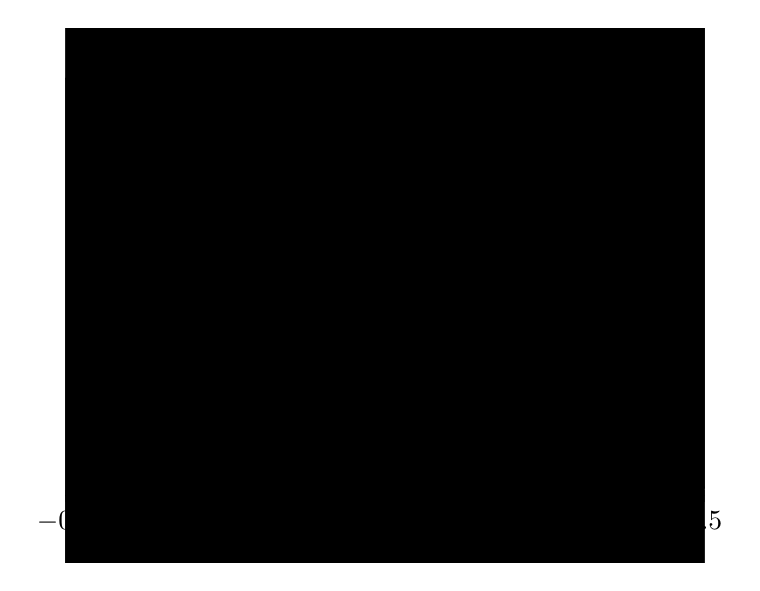
\begin{tikzpicture}
  \begin{axis}[
      axis lines = middle,
      xlabel = $X$,
      ylabel = $Y$,
      width=0.8\textwidth,
      variable=t
  ]

  \draw [line width=0.2mm, dashed] (axis cs:0,2) -- (axis cs:2,2) -- (axis cs:2,0);
  \draw [line width=0.1mm] (axis cs:1,1) -- (axis cs:3,1) -- (axis cs:3,3) -- (axis cs:1,3) -- (axis cs:1,1);

  \draw [fill=black] (axis cs:2,0)  circle (4) node[above right] {$\EE_X$};
  \draw [fill=black] (axis cs:0,2)  circle (4) node[above right] {$\EE_Y$};
  \draw [fill=black] (axis cs:2,2)  circle (4);

  \draw[rotate around={55: (axis cs:2, 2)}, dashed] (axis cs:2, 2) ellipse (1.3cm and 2.4cm);
  \addplot [draw=none, forget plot] coordinates {(1.6,2.6)} node {$Cov(X,Y)$};

  \draw [line width=0.2mm, decorate,decoration={snake,amplitude=.4mm,segment length=2mm,post length=0mm}] (axis cs:0,1) -- (axis cs:0,3);
  \draw [line width=0.2mm, decorate,decoration={snake,amplitude=.4mm,segment length=2mm,post length=0mm}] (axis cs:1,0) -- (axis cs:3,0);

  \addplot [draw=none, forget plot] coordinates {(3.5, 3.5)};
  \addplot [draw=none, forget plot] coordinates {(-0.5, -0.5)};

  \end{axis}
  \end{tikzpicture}
  \caption{covarianza (negativa) per due VA}\label{fig-covarianza}
\end{figure}

\subsubsection{Indipendenza e scorrelazione}

\begin{teob}[\JPTh{12.3}]\label{teo-correl}
  \index{scorrelazione}
  Siano $X,Y \in L^2(\PP)$ tali che $X \indep Y$. Allora $Cov(X,Y) = 0.$ \\
  Due variabili che hanno covarianza nulla di dicono \emph{scorrelate}.
\end{teob}

\begin{dimo}
  Per $X, Y$ limitate (che infatti sono in $L^2$):
  $$ Cov(X,Y) = \Ex{XY} - \Ex{X} \Ex{Y} \stackrel{X \indep Y}{=} \Ex{X} \Ex{Y} - \Ex{X} \Ex{Y} = 0. $$
  Per $X,Y$ illimitate l'uguaglianza è comunque verificata costruendo due successioni crescenti ${X_n}, {Y_n}$ che tendono, rispettivamente, a $X$ e a $Y$; la convergenza dominata garantisce la possibilità di scambiare limite e valore atteso. \qedhere
\end{dimo}

\medskip
\begin{nb}
  In generale, il viceversa del teorema \emph{non è vero}!
  $$Cov(X,Y) = 0 \centernot\implies X \indep Y$$
  L'indipendenza è una condizione più forte della correlazione; ovvero, esistono coppie di variabili scorrelate ma non indipendenti. Più avanti entreremo più in dettaglio sul significato della (s)correlazione.
\end{nb}

\medskip
\begin{ese}
  Consideriamo una probabilità concentrata su 4 punti, ovvero:
  $$(X,Y) \sim U( \{ (\pm 1, 0), (0, \pm 1) \} )$$

  \begin{figure}[ht]
    \centering
    \begin{tikzpicture}
    \begin{axis}[
      axis lines = middle,
      xlabel = $X$,
      ylabel = {$Y$},
      width=0.5\textwidth,
      height=0.5\textwidth,
    ]

    \addplot [draw=none, forget plot] coordinates {(-1.4,-1.4)};
    \addplot [draw=none, forget plot] coordinates {(1.4, 1.4)};

    \addplot [only marks, mark=*] table {
      1 0
      0 1
      -1 0
      0 -1
      };

    \end{axis}
    \end{tikzpicture}
    \caption{VA $(X,Y)$ concentrata su 4 punti}\label{fig-prob-concentrata}
  \end{figure}

  La figura \ref{fig-prob-concentrata} è simmetrica rispetto all'origine, nel senso che non c'è allungamento in una delle direzioni diagonali, quindi $Cov(X,Y) = 0$ (risultato che, peraltro, si può anche verificare con rapidi conti).
  Tuttavia $X \centernot\indep Y$ perché la figura non forma un rettangolo. Infatti, prendendo una sezione qualsiasi dell'``area'' in cui è condensata la probabilità, si osserva immediatamente che conoscere un'informazione su una delle due variabili (per esempio $X=1$) può influenzare il grado di fiducia sull'altra (per esempio è vero che $\PP(Y = 0 \, | \, X = 1) = 1$).

  Due VA sono indipendenti se e solo se il grafico del supporto (ovvero l'insieme dei punti in cui è condensata la probabilità) forma un rettangolo, sia esso discreto (come in questo caso) o continuo. Infatti prendendo una sezione del rettangolo, ovvero fissando un valore di una delle due VA, il grado di fiducia dell'altra VA non cambia perché il segmento-sezione ha ugual lunghezza lungo tutto il supporto.
\end{ese}

\medskip
\begin{ese}
  Consideriamo il cerchio $S = \{ (x,y) \in \RR^2 : x^2 + y^2 \leq 1 \}$ e il vettore aleatorio $(X,Y) \sim U(S)$. \\
  Notiamo immediatamente che $(X, Y)$ ha probabilità concentrata su $S$.

  Anche qui $Cov(X,Y) = 0$ per simmetria centrale, ma $X \centernot\indep Y$ perché il supporto non è un rettangolo. Verifichiamo questa conclusione mostrando un punto in cui le probabilità non si fattorizzano, per esempio:
  $$\PP \left(Y \geq \frac{1}{2} | X = 1 \right) = 0 \neq \PP \left(Y \geq \frac{1}{2} \right)$$
\end{ese}

\medskip
\begin{prop}
  $$|Cov(X,Y)| \leq \sqrt{Var(X) \, Var(Y)}$$
\end{prop}
La proposizione è un'immediata conseguenza della disuguaglianza di Cauchy-Schwarz.

\subsubsection{Coefficiente di correlazione lineare}

\begin{defn}
  \index{coefficiente di correlazione lineare}
  Siano $X$ e $Y$ VAR su $\DoCo[1]$ in $L^2(\PP)$ e tali che $Var(X)>0$ e $Var(Y)>0$.
  Si definisce \textbf{coefficiente di correlazione lineare} il valore:
  $$\rho \coloneqq \frac{Cov(X,Y)}{\sqrt{Var(X) \, Var(Y)}}$$
\end{defn}
Sappiamo che $|\rho| \leq 1$ per la proposizione precedente e che $X \indep Y \implies \rho = 0$ per il teorema \ref{teo-correl}. \\
Notiamo inoltre che $\rho$ è adimensionale in quanto indica un rapporto tra grandezze omogenee, al contrario di media, varianza e altri oggetti probabilistici.

\medskip
\begin{prop}
  Siano $X,Y \in L^2(\PP)$ tali che $Var(X)>0$ e $Var(Y)>0$. \\
  Si ha $|\rho| = 1$ se e solo se esistono $a, b \in \RR, a \neq 0,$ tali che $Y = aX + b$. In tal caso, vale:
    $$Y =
    \rho \sqrt{\dfrac{Var(Y)}{Var(X)}}X + \Ex{Y} -
    \rho \sqrt{\dfrac{Var(X)}{Var(Y)}} \Ex{X}$$
\end{prop}

Il risultato (1) è coerente con quanto precedentemente detto sulla covarianza. Una covarianza positiva (o negativa) indica infatti una distribuzione di punti stretta e allungata nella direzione I-III (o II-IV) quadrante, e il caso $|\rho| = 1$ indica il caso estremo di questo stringimento e allungamento: tutti i punti si allineano su una retta, che, per inciso, permette di calcolare deterministicamente il valore di $Y = aX + b = h(X)$; questo infatti è il caso opposto rispetto all'indipendenza tra due VA (dove infatti $Cov(X,Y) = 0$).

% to-do: Gioele sei arrivato qua
\smallskip
\begin{dimo}
  %Il punto 1. sarà dimostrato a esercitazione.\footnote{Spudorata menzogna, è stato lasciato come esercizio individuale}\\
  %%to-do: è a questa schifezza qui a cui mi riferivo
  %%noto-do: Esticazzi (AW)
  %L'ho lasciato perché è troppo bello per essere cancellato davvero (Br1)
  Sarà dimostrato solo il punto (2). Sapendo che da $Y = aX + b$ discendono $Var(Y) = a^2 Var(X)$ e $\Ex{Y} = a \Ex{X} + b$, è sufficiente sostituire nella formula queste due espressioni per verificare facilmente che danno un'identità.
\end{dimo}
\begin{nb}
  I casi in cui $Y$ è espresso come una retta orizzontale o verticale (rispetto a un sistema di riferimento $OXY$) andrebbero studiati a parte, ma sono comunque di facile trattazione e non costituiscono dunque un ostacolo alla generalità della proposizione.
\end{nb}
\subsubsection{Proprietà}

\begin{prop}
  \index{bilinearità della covarianza}
  La covarianza è \textit{bilineare}, ovvero lineare su entrambi gli argomenti:
  \begin{align*}
    Cov&(aX+bY,cZ+dW) = \\
    &= ac \cdot Cov(X,Z) + ad \cdot Cov(X,W) + bc \cdot Cov(Y,Z) + bd \cdot Cov(Y,W)
  \end{align*}
\end{prop}
La dimostrazione è banale ma non immediata: si effettua con noiosi conti su $Cov(aX+bY, Z)$. Per simmetria la proposizione sarà dunque vera anche per l'altro argomento, senza necessità di complicare ulteriormente i calcoli.

\begin{coro}
  $$Var(X+Y) = Var(X) + Var(Y) + 2 Cov(X,Y)$$
\end{coro}
La dimostrazione è banale e immediata calcolando $Var(X+Y)$ come $Cov(X+Y,X+Y)$.

\subsection{Vettore media e matrice varianza}

\begin{defn}
  \index{valore atteso!in $\RR^n$}
  \index{vettore media (valore atteso)}
  Sia $X = (X_1, \, \dots, \, X_n): \DoCo$ un vettore aleatorio. \\
  Il \textbf{vettore media} di $X$, se le componenti sono $L^1$, è il vettore delle medie delle componenti:
  $$ \Ex{X} \coloneqq \begin{bmatrix} \Ex{X_1} \\ \vdots \\ \Ex{X_n} \end{bmatrix} $$
  \index{matrice varianza}
  e, se le componenti sono $L^2$, la \textbf{matrice varianza}, o matrice delle covarianze, di $X$ è:
  $$ C \coloneqq
  \begin{bmatrix} Var(X_1)    & \dots   & Cov(X_1, X_n) \\
          \vdots      & \ddots  & \vdots \\
          Cov(X_n, X_1)   & \dots   & Var(X_n)
  \end{bmatrix}
  \text{ ovvero } C_{ij} = Cov(X_i, X_j)$$
\end{defn}

\medskip
\begin{teob}[\JPTh{12.4}]
  \index{semi-definita positività}
  Sia $X$ vettore aleatorio con componenti $X_1, \, \dots, \, X_n \in L^2$. \\
  Allora $C$ è \textit{semi-definita positiva}\footnote{Si noti che in questo corso si include la simmetria della matrice nella definizione di semi-definita positività, sebbene in altri testi e corsi sia trattata come una proprietà a parte.}
  (indicato con $C \geq 0$), ovvero:
  $$ C = C^T \qquad \text{e} \qquad a^T C a \geq 0 \ \ \forall a = (a_1, \, \dots, \, a_n) \in \RR^n$$
\end{teob}

\begin{dimo}\belowdisplayskip=-21pt
  La simmetria è ovvia perché $Cov(X,Y) = Cov(Y,X)$. \\
  Grazie alla bilinearità della covarianza si ha:
  \begin{align*}
    a^T C a
    &= \sum_{i,j} a_i C_{ij} a_j & (\text{scomponendo i vettori})\\
    &= \sum_{i,j} a_i Cov(X_i, X_j)  a_j & (\text{passando alle covarianze})\\
    &= \sum_i \sum_j Cov(a_i X_i, a_j X_j) & (\text{per bilinearità})\\
    &= Cov\left( \sum_i a_i X_i, \sum_j a_j X_j\right) & (\text{per bilinearità})\\
    &= Var\left(\sum_i a_i X_i\right) \geq 0 \quad \forall a \in \RR^n
  \end{align*}\qedhere
\end{dimo}
\bigskip
\begin{teo} \label{appartenenza VeAle}
    Sia $X$ vettore aleatorio con componenti $X_1, \, \dots, \, X_n \in L^2$.
    Allora:
    $$X \in \operatorname{range}(C) + \Ex X \text \enspace {\text{ qc}}$$
    Qui $\operatorname{range}(C) = \operatorname{col}(C)$ è lo spazio colonna di $C$, ovvero lo spazio vettoriale avente come base le colonne di $C$.
\end{teo}
Lo spazio indicato dal teorema è uno \textit{spazio affine} di $\RR^n$, ovvero ottenuto mediante una trasformazione lineare (la matrice $C$) e una traslazione (l'aggiunta di $\Ex{X}$). \\
Si noti inoltre che è possibile che $X$ non possa assumere tutti i valori di $\RR^n$; ciò succede nel caso in cui due o più colonne di $C$ sono linearmente dipendenti, ovvero se la matrice non ha rango massimo.

Questo teorema ha un'importante conseguenza.
\begin{coro}
	Se $X$ è un vettore aleatorio continuo, allora la sua matrice varianza $C$ è invertibile;
	equivalentemente, se $C$ non è invertibile allora $X$ non è continuo.
	%Mi sembra inutile specificare questa seconda parte, visto che è completamente ovvia dalla prima; la teniamo? (Br1)
	%Io la lascerei comunque, non fa male (SSL)
\end{coro}
Si noti che questa condizione è solo necessaria e non sufficiente.
Per esempio, si può verificare che il controesempio mostrato a pagina \pageref{cese-parabola-normale}, cioè $W = (X,X^2)$ con $X \sim \Nc(0,1)$, ha matrice varianza $C$ invertibile pur non essendo continuo.

\medskip
\begin{teob}[\JPTh{12.5}]
  Siano $X: \DoCo$ un vettore aleatorio con varianza $C_X$, e
  $Y = AX+b$ un vettore aleatorio, con $A \in \RR^{m \times n}$ e $b \in \RR^m$. Allora:
  $$ \Ex{Y} = A \ \Ex{X} + b \quad \text{e} \quad C_Y = A \, C_X \, A^T$$
\end{teob}
Quest'ultima formula è molto utile in contesti pratici per ridurre le dimensioni dei vettori, al fine di facilitare i conti.
\begin{dimo}\Fixvmode
	\begin{enumerate}
	\item Calcoliamo la $i$-esima componente del vettore media sfruttando la linearità del valore atteso:
	$$\EE[Y_i] = \EE\left[ \sum_j a_{ij} X_j + b_i \right] = \sum_j a_{ij} \EE[X]_j + b_i = (A \, \EE[X] + b)_i$$
	\item Per quanto riguarda la matrice varianza:
	\begin{align*}
		(C_Y)_{ij} &=Cov(Y_i,Y_j) \\
		&=Cov \left(\sum_k a_{ik} X_k + b_i, \ \sum_m a_{jm} X_m +b_j \right) \\
		&=\sum_{k,m} a_{ik} a_{jm} (C_X)_{ij} &\text{(bilinearità)} \\
		&= (A \, C_X \, A^T)_{ij} & \qedhere
	\end{align*}
	\end{enumerate}
\end{dimo}

\cleardoublepage
